\documentclass[12pt,a4paper]{article}

% ============================================
% PACKAGES
% ============================================
\usepackage[utf8]{inputenc}
\usepackage[T1]{fontenc}
\usepackage[french]{babel}
\usepackage{amsmath, amsfonts}
\usepackage{graphicx}
\usepackage{float}
\usepackage{booktabs}
\usepackage{geometry}
\usepackage{xcolor}
\usepackage{listings}
\usepackage{hyperref}
\usepackage{fancyhdr}

% ============================================
% CONFIGURATION
% ============================================
\geometry{left=2.5cm, right=2.5cm, top=2.5cm, bottom=2.5cm}
\hypersetup{colorlinks=true, linkcolor=blue, urlcolor=cyan}

% Configuration des listings
\lstdefinestyle{Rstyle}{
    language=R,
    basicstyle=\ttfamily\footnotesize,
    keywordstyle=\color{blue}\bfseries,
    commentstyle=\color{green!60!black},
    numbers=left,
    numberstyle=\tiny\color{gray},
    backgroundcolor=\color{gray!10},
    frame=single,
    breaklines=true,
    tabsize=2
}

\lstdefinestyle{Pythonstyle}{
    language=Python,
    basicstyle=\ttfamily\footnotesize,
    keywordstyle=\color{blue}\bfseries,
    commentstyle=\color{green!60!black},
    numbers=left,
    numberstyle=\tiny\color{gray},
    backgroundcolor=\color{yellow!10},
    frame=single,
    breaklines=true,
    tabsize=4
}

% En-tête
\pagestyle{fancy}
\fancyhf{}
\rhead{GMM2 - Exercice 2}
\lhead{Analyse Factorielle des Correspondances}
\cfoot{\thepage}

% ============================================
% DOCUMENT
% ============================================
\begin{document}

% ============================================
% TITRE
% ============================================
\begin{center}
    \rule{\linewidth}{0.5mm}\\[0.4cm]
    {\Huge \textbf{EXERCICE 2}}\\[0.3cm]
    {\Large \textbf{Analyse Factorielle des Correspondances (AFC)}}\\[0.2cm]
    {\large Base de données : Housetasks}\\[0.1cm]
    \rule{\linewidth}{0.5mm}\\[1cm]
\end{center}

% ============================================
% PRÉSENTATION DES DONNÉES
% ============================================
\section{Présentation des Données}

\subsection{Description}

La base de données \textbf{Housetasks} présente la répartition des tâches ménagères au sein des couples. Il s'agit d'une \textbf{table de contingence} croisant :
\begin{itemize}
    \item \textbf{11 tâches ménagères} (en lignes) : Cooking, Laundry, Cleaning, Shopping, Ironing, Finances, Repairs, Driving, Gardening, Homework, Dishes
    \item \textbf{4 modalités de réalisation} (en colonnes) : Wife (épouse), Alternating (alternance), Husband (époux), Jointly (ensemble)
\end{itemize}

\subsection{Table de contingence}

\begin{table}[H]
\centering
\caption{Table de contingence des tâches ménagères}
\begin{tabular}{|l|c|c|c|c|c|}
\hline
\textbf{Tâche} & \textbf{Wife} & \textbf{Alternating} & \textbf{Husband} & \textbf{Jointly} & \textbf{Total} \\
\hline
Cooking & 156 & 14 & 4 & 2 & 176 \\
Laundry & 124 & 20 & 12 & 23 & 179 \\
Cleaning & 77 & 11 & 13 & 21 & 122 \\
Shopping & 82 & 36 & 11 & 52 & 181 \\
Ironing & 53 & 11 & 2 & 13 & 79 \\
Finances & 32 & 24 & 10 & 9 & 75 \\
Repairs & 33 & 23 & 9 & 17 & 82 \\
Driving & 12 & 8 & 7 & 6 & 33 \\
Gardening & 10 & 7 & 15 & 5 & 37 \\
Homework & 7 & 11 & 14 & 4 & 36 \\
Dishes & 13 & 15 & 20 & 11 & 59 \\
\hline
\textbf{Total} & \textbf{599} & \textbf{180} & \textbf{117} & \textbf{163} & \textbf{1059} \\
\hline
\end{tabular}
\end{table}

\subsection{Statistiques descriptives}

\subsubsection{Répartition globale par responsable}

\begin{table}[H]
\centering
\caption{Répartition globale des tâches par responsable}
\begin{tabular}{|l|c|c|}
\hline
\textbf{Responsable} & \textbf{Effectif} & \textbf{Pourcentage} \\
\hline
Wife (Épouse) & 599 & 56.6\% \\
Alternating (Alternance) & 180 & 17.0\% \\
Husband (Époux) & 117 & 11.0\% \\
Jointly (Ensemble) & 163 & 15.4\% \\
\hline
\textbf{Total} & \textbf{1059} & \textbf{100\%} \\
\hline
\end{tabular}
\end{table}

\textbf{Observation :} L'épouse réalise plus de la moitié (56.6\%) de l'ensemble des tâches ménagères, tandis que l'époux n'en assume que 11\%. Les tâches partagées (Jointly + Alternating) représentent environ 32\% du total.

\subsubsection{Profil de chaque tâche}

\begin{table}[H]
\centering
\caption{Pourcentage de réalisation par tâche et par responsable}
\footnotesize
\begin{tabular}{|l|c|c|c|c|c|}
\hline
\textbf{Tâche} & \textbf{Total} & \textbf{Wife (\%)} & \textbf{Husband (\%)} & \textbf{Jointly (\%)} & \textbf{Alternating (\%)} \\
\hline
Cooking & 176 & \textbf{88.6} & 2.3 & 1.1 & 8.0 \\
Laundry & 179 & \textbf{69.3} & 6.7 & 12.8 & 11.2 \\
Cleaning & 122 & \textbf{63.1} & 10.7 & 17.2 & 9.0 \\
Ironing & 79 & \textbf{67.1} & 2.5 & 16.5 & 13.9 \\
Shopping & 181 & 45.3 & 6.1 & \textbf{28.7} & 19.9 \\
Finances & 75 & 42.7 & 13.3 & 12.0 & \textbf{32.0} \\
Repairs & 82 & 40.2 & 11.0 & 20.7 & 28.0 \\
Driving & 33 & 36.4 & 21.2 & 18.2 & 24.2 \\
Gardening & 37 & 27.0 & \textbf{40.5} & 13.5 & 18.9 \\
Homework & 36 & 19.4 & \textbf{38.9} & 11.1 & 30.6 \\
Dishes & 59 & 22.0 & \textbf{33.9} & 18.6 & 25.4 \\
\hline
\end{tabular}
\end{table}

\textbf{Observations clés :}
\begin{itemize}
    \item \textbf{Tâches très féminines} : La cuisine (88.6\%), la lessive (69.3\%) et le repassage (67.1\%) sont majoritairement réalisés par l'épouse.
    \item \textbf{Tâches plutôt masculines} : Le jardinage (40.5\%), les devoirs (38.9\%) et la vaisselle (33.9\%) montrent une prédominance du mari.
    \item \textbf{Tâches partagées} : Les courses (28.7\% ensemble) et les finances (32\% en alternance) sont les plus équitablement réparties.
\end{itemize}

% ============================================
% MÉTHODOLOGIE
% ============================================
\section{Méthodologie}

L'\textbf{Analyse Factorielle des Correspondances (AFC)} est une méthode adaptée à l'analyse des tables de contingence. Elle permet de :

\begin{enumerate}
    \item Étudier les \textbf{associations} entre les modalités lignes et colonnes
    \item Représenter graphiquement ces associations sur un \textbf{biplot}
    \item Mesurer l'\textbf{écart à l'indépendance} entre les variables
\end{enumerate}

\textbf{Principe :} L'AFC décompose l'\textbf{inertie totale} (liée au $\chi^2$) en axes factoriels orthogonaux, permettant de visualiser les proximités entre modalités.

% ============================================
% RÉSULTATS
% ============================================
\section{Résultats}

\subsection{Test d'indépendance}

\begin{table}[H]
\centering
\caption{Résultats du test du Chi-deux}
\begin{tabular}{|l|c|}
\hline
\textbf{Statistique} & \textbf{Valeur} \\
\hline
Chi-deux ($\chi^2$) & 279.27 \\
Degrés de liberté & 30 \\
p-value & $3.11 \times 10^{-42}$ \\
Inertie totale & 0.2637 \\
\hline
\end{tabular}
\end{table}

\textbf{Interprétation :} La p-value extrêmement faible ($< 0.001$) indique un \textbf{rejet de l'hypothèse d'indépendance}. Il existe donc une association statistiquement significative entre les tâches ménagères et la personne qui les réalise.

\subsection{Résultats de l'AFC}

\begin{figure}[H]
    \centering
    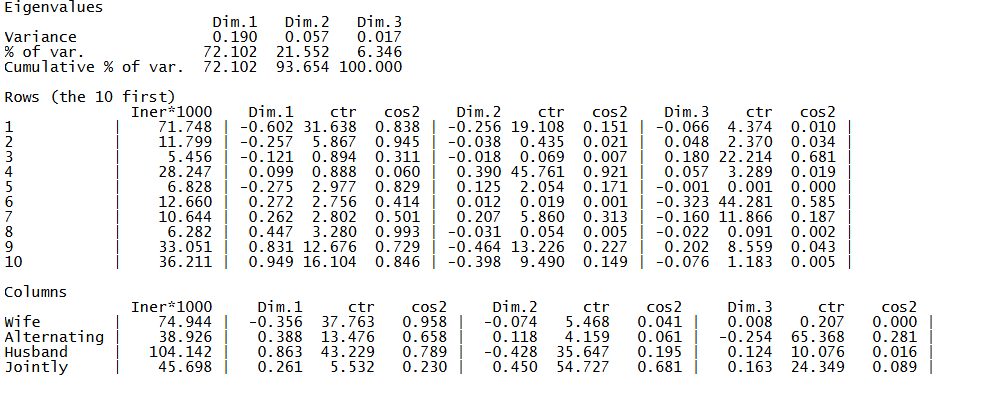
\includegraphics[width=0.95\textwidth]{AFC_resultats.png}
    \caption{Résultats numériques de l'AFC (valeurs propres, coordonnées, contributions)}
    \label{fig:afc_resultats}
\end{figure}

\subsection{Biplot de l'AFC}

\begin{figure}[H]
    \centering
    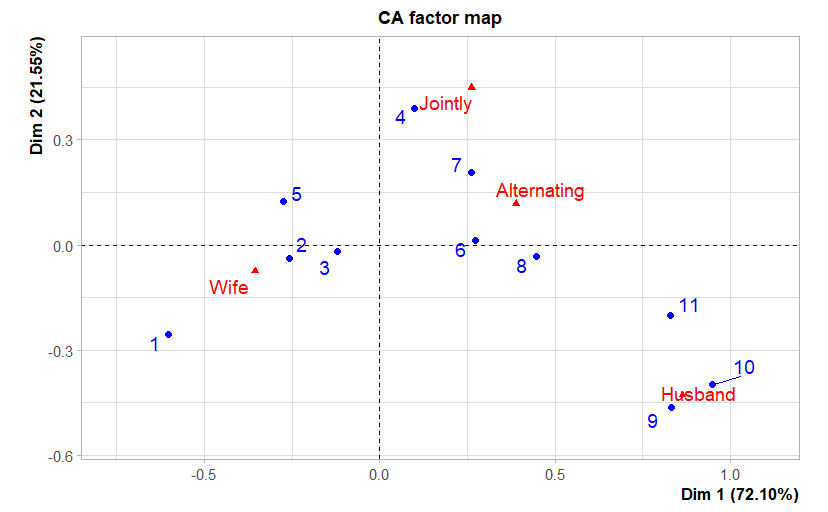
\includegraphics[width=0.9\textwidth]{Plot_AFC.png}
    \caption{Représentation simultanée des tâches et des modalités (Biplot AFC)}
    \label{fig:biplot}
\end{figure}

% ============================================
% INTERPRÉTATION
% ============================================
\section{Interprétation des Résultats}

\subsection{Interprétation des axes factoriels}

\subsubsection{Axe 1 : Opposition Épouse / Époux}

Le premier axe factoriel, qui explique la plus grande partie de l'inertie, représente l'\textbf{opposition fondamentale entre les rôles de genre} dans la répartition des tâches ménagères :

\begin{itemize}
    \item \textbf{Côté négatif (gauche)} : On retrouve la modalité \textbf{"Wife"} ainsi que les tâches traditionnellement féminines comme la \textbf{cuisine} (Cooking), la \textbf{lessive} (Laundry) et le \textbf{repassage} (Ironing). Ces tâches sont caractérisées par une très forte proportion de réalisation par l'épouse (entre 67\% et 89\%).
    
    \item \textbf{Côté positif (droite)} : On trouve la modalité \textbf{"Husband"} accompagnée des tâches comme le \textbf{jardinage} (Gardening), les \textbf{devoirs} (Homework) et la \textbf{vaisselle} (Dishes). Ces activités montrent une participation masculine plus importante que la moyenne.
\end{itemize}

Cet axe met en évidence la persistance d'une \textbf{division sexuée du travail domestique}, où les tâches d'intérieur (cuisine, ménage, linge) restent majoritairement féminines, tandis que les tâches d'extérieur ou techniques tendent vers le masculin.

\subsubsection{Axe 2 : Tâches individuelles vs partagées}

Le deuxième axe factoriel apporte une information complémentaire en distinguant :

\begin{itemize}
    \item \textbf{Partie supérieure} : Les tâches réalisées de manière \textbf{individuelle} par un seul membre du couple. On y trouve notamment la cuisine (très exclusivement féminine avec 88.6\%) et le jardinage (principalement masculin avec 40.5\%).
    
    \item \textbf{Partie inférieure} : Les modalités \textbf{"Jointly"} (ensemble) et \textbf{"Alternating"} (alternance), accompagnées des tâches comme les \textbf{courses} (Shopping) et les \textbf{finances}. Ces activités représentent les domaines où le couple tend vers un partage plus équitable des responsabilités.
\end{itemize}

\subsection{Analyse détaillée du biplot}

Le biplot (Figure \ref{fig:biplot}) offre une visualisation synthétique des associations entre tâches et responsables. L'interprétation repose sur la \textbf{proximité géométrique} : plus deux points sont proches, plus leur association est forte.

\subsubsection{Tâches fortement associées à l'épouse (Wife)}

\begin{itemize}
    \item \textbf{Cooking (Cuisine)} : Avec 88.6\% de réalisation par l'épouse, c'est la tâche la plus genrée de l'étude. Sur le biplot, elle apparaît très proche du point "Wife" et éloignée de toutes les autres modalités. Cela reflète une norme sociale encore très ancrée où la préparation des repas incombe principalement aux femmes.
    
    \item \textbf{Laundry (Lessive)} : 69.3\% par l'épouse. Cette tâche de gestion du linge reste fortement féminisée, ce qui s'explique historiquement par la division des espaces domestiques.
    
    \item \textbf{Ironing (Repassage)} : 67.1\% par l'épouse. Tâche complémentaire à la lessive, elle suit le même schéma de répartition.
    
    \item \textbf{Cleaning (Ménage)} : 63.1\% par l'épouse. L'entretien général du foyer reste une responsabilité majoritairement féminine.
\end{itemize}

\subsubsection{Tâches associées à l'époux (Husband)}

\begin{itemize}
    \item \textbf{Gardening (Jardinage)} : 40.5\% par l'époux, la plus forte proportion masculine. Cette tâche d'extérieur correspond à une activité traditionnellement masculine liée à l'espace public.
    
    \item \textbf{Homework (Devoirs)} : 38.9\% par l'époux. Fait intéressant, l'aide aux devoirs des enfants montre une implication paternelle significative.
    
    \item \textbf{Dishes (Vaisselle)} : 33.9\% par l'époux. Contrairement à la cuisine, la vaisselle apparaît comme une tâche plus partagée.
    
    \item \textbf{Driving (Conduite)} : 21.2\% par l'époux. Les déplacements en voiture montrent une tendance masculine, bien que moins marquée.
\end{itemize}

\subsubsection{Tâches partagées (Jointly / Alternating)}

\begin{itemize}
    \item \textbf{Shopping (Courses)} : Avec 28.7\% réalisé conjointement et 19.9\% en alternance, les courses représentent l'activité la plus équitablement partagée. Cela peut s'expliquer par le caractère familial et social de cette sortie.
    
    \item \textbf{Finances} : 32\% en alternance. La gestion du budget familial tend vers un partage des responsabilités, reflétant l'évolution vers une égalité dans les décisions économiques du foyer.
    
    \item \textbf{Repairs (Réparations)} : Bien que souvent perçues comme masculines, les réparations montrent 20.7\% de réalisation conjointe, suggérant une certaine collaboration.
\end{itemize}

\subsection{Synthèse de l'interprétation}

L'AFC appliquée aux données Housetasks révèle plusieurs enseignements majeurs :

\begin{enumerate}
    \item \textbf{Persistance des stéréotypes de genre} : La répartition des tâches ménagères reste largement influencée par les rôles traditionnels. L'épouse assume 56.6\% de l'ensemble des tâches, contre seulement 11\% pour l'époux.
    
    \item \textbf{Dichotomie intérieur/extérieur} : Les tâches d'intérieur (cuisine, ménage, linge) sont féminines, tandis que les activités d'extérieur ou techniques (jardinage, réparations) tendent vers le masculin.
    
    \item \textbf{Émergence du partage} : Certaines tâches comme les courses et la gestion financière montrent une évolution vers un partage plus équitable, témoignant d'une modernisation progressive des rapports de couple.
    
    \item \textbf{Charge mentale inégale} : La concentration des tâches quotidiennes et répétitives (cuisine, ménage) chez l'épouse suggère une charge mentale domestique disproportionnée.
\end{enumerate}

% ============================================
% CODES
% ============================================
\section{Codes R et Python}

\subsection{Code R}

\begin{lstlisting}[style=Rstyle, caption={Code R pour l'AFC avec FactoMineR}]
# Charger les librairies
library(readxl)
library(FactoMineR)

# Charger les donnees
housetasks <- read_excel("housetasks.xlsx")
Data <- housetasks

# Table de Contingence (supprimer colonne des noms)
DataAFC <- Data[, -1]

# Executer l'AFC
CAResults1 <- CA(DataAFC, graph = FALSE)

# Afficher les resultats
summary(CAResults1)

# Modifier les noms des lignes
rownames(CAResults1$row$coord) <- c("Cooking", "Laundry", 
    "Cleaning", "Shopping", "Ironing", "Finances", 
    "Repairs", "Driving", "Gardening", "Homework", "Dishes")

# Visualiser le biplot
plot.CA(CAResults1, axes = c(1, 2))
\end{lstlisting}

\subsection{Code Python}

\begin{lstlisting}[style=Pythonstyle, caption={Code Python pour l'AFC}]
import pandas as pd
import numpy as np
import matplotlib.pyplot as plt
from scipy import stats

# Charger les donnees
ht = pd.read_excel("housetasks.xlsx")

# Table de contingence
contingency = ht.iloc[:, 1:].values
row_names = ht.iloc[:, 0].values
col_names = ht.columns[1:].tolist()

# Test du Chi2
chi2, p, dof, expected = stats.chi2_contingency(contingency)
print(f"Chi2 = {chi2:.2f}, p-value = {p:.2e}")

# Inertie totale
grand_total = contingency.sum()
inertia = chi2 / grand_total
print(f"Inertie totale = {inertia:.4f}")

# Pour l'AFC complete, utiliser le package 'prince':
# pip install prince
# import prince
# ca = prince.CA(n_components=2)
# ca = ca.fit(pd.DataFrame(contingency, 
#             index=row_names, columns=col_names))
# ca.plot_coordinates(figsize=(10, 8))
\end{lstlisting}

% ============================================
% CONCLUSION
% ============================================
\section{Conclusion}

L'AFC appliquée aux données Housetasks met en évidence :
\begin{enumerate}
    \item Une \textbf{dépendance significative} entre tâches ménagères et responsables ($\chi^2 = 279.27$, $p < 0.001$)
    \item Une \textbf{répartition traditionnelle} des rôles : tâches domestiques pour l'épouse, bricolage/extérieur pour l'époux
    \item L'émergence de \textbf{tâches partagées} (courses, finances) reflétant une évolution des mœurs
\end{enumerate}

\end{document}
